\documentclass[a4paper,14pt]{ctexart}
\CTEXsetup[format+={\flushleft}]{section}
\usepackage{wrapfig}
\usepackage{lipsum} 
\linespread{1.05} % Line spacing - Palatino needs more space between lines
\usepackage{microtype} % Slightly tweak font spacing for aesthetics
\usepackage{texnames}
\usepackage[hmarginratio=1:1,top=32mm,columnsep=20pt]{geometry} % Document margins

\usepackage[hang, small,labelfont=bf,up,textfont=it,up]{caption} % Custom captions under/above floats in tables or figures
\usepackage{booktabs} % Horizontal rules in tables
\usepackage{float} % Required for tables and figures in the multi-column environment - they need to be placed in specific locations with the [H] (e.g. \begin{table}[H])

\usepackage[colorlinks,linkcolor=black,anchorcolor=black,citecolor=black,urlcolor=black]{hyperref}
%\usepackage{hyperref}

\usepackage{graphicx}
\usepackage{paralist} % Used for the compactitem environment which makes bullet points with less space between them
\usepackage{float}


\usepackage{fancyhdr} % Headers and footers
\pagestyle{fancy} % All pages have headers and footers
\fancyhead{} % Blank out the default header
\fancyfoot{} % Blank out the default footer
%\fancyhead[C]{Running title $\bullet$ March 2015} % Custom header text
\fancyfoot[RO,LE]{\thepage} % Custom footer text



\title{\vspace{-15mm}\fontsize{24pt}{10pt}\selectfont\textbf{需求分析说明书}\protect\\ \vspace{5mm} \Large ——在线摄影约拍平台} 


\author{
\large
\textsc{Team 15}\thanks{南京大学计算机科学与技术系,软件工程小组,组长:肖少东(121220109)。组员:向根(121220107),向耀程(121220108),姚开浪(121220120),张晗(121220135)。本文通过 \LaTeX 编写。}\\[2mm] 
\normalsize 南京大学计算机科学与技术系 \\
\normalsize version 1.2 (添加UML模型)
}
\date{2015年 3月}



\begin{document}

\maketitle 

\tableofcontents

\thispagestyle{fancy}


\newpage
\section{引言}

\subsection{编写目的}
 该需求分析说明书用于定义和描述在线摄影约拍平台的功能特性和用户需求说明,并对约拍网在运营过程中可能出现的故障或问题提出了相应的解决办法。在线摄影约拍网站“影南忘”旨在为摄影爱好者提供无缝对接的约拍平台,通过用户登陆注册为摄影师或模特,经由轻社交模式互动,实现对所需摄影师或模特的筛选,进而促成线下约拍合作。
\subsection{背景}
软件初步定名为“影南忘”——在线摄影约拍平台(目前已有微信公众号,订阅用户逾1千)。\par

随着人们生活水平的提高,高端摄影设备已被越来越多的普通爱好者所拥有。定制人像摄影作为摄影类型的一个大类,吸引越来越多的专业摄影师和摄影爱好者进行商业或非商业的约拍行为。然而,传统的线上约拍方式借助社交网络或兴趣论坛,线上到线下转化率低、流程不透明、时间成本高昂,因此便产生了对于一个专业摄影约拍网站的需求。而这正是我们要做的。




\section{任务概述}
\begin{figure}[H]
\centering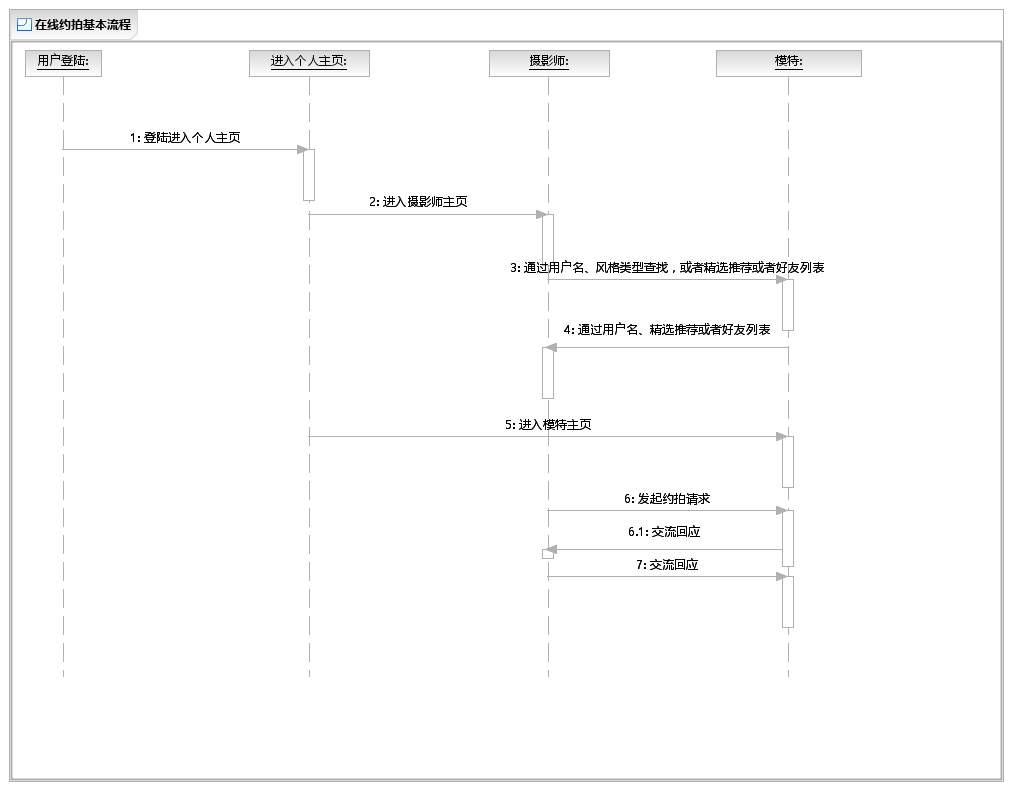
\includegraphics[width=4.5in]{时序图-约拍.jpeg}
\caption{时序图:约拍}
\label{fig:13}
\end{figure}
\subsection{目标}
在线摄影约拍平台极大降低了约拍的时间成本,提高了目标指向性。任何人都能够以摄影师或模特身份申请用户账号,并拥有个人主页。成为注册用户后,可对已注册的摄影师或模特进行条件搜索。在找到中意的摄影师或模特后,进入其个人主页,即可看到其联系方式或对其发送私信。\par
每个注册用户都拥有可发布图文信息的个人主页。用户亦可关注喜爱的摄影师或模特,对被关注者的博客或内容进行评论和点赞。\par


\subsection{用户描述}
网站建成后,未注册登录用户,可进行首页浏览,看到首页精选内容。但不具备搜索摄影师模特,关注他人个人主页的权限功能。\par
任何人都可以注册成为网站注册用户,注册用户分为摄影师和模特两类。两类用户具备基本相同的权限,包括拥有个人主页并发布图文内容、关注其他摄影师或模特的博客。摄影师和模特的个人主页会通过特殊符号标识进行区别,且显示在个人主页上的信息条目有所差异。\par
管理员用户具备后台管理权限,须具有判断图文信息是否符合互联网信息传播规定的能力。管理员有权限关闭某非法注册用户的个人主页,有权限删除某条不符合互联网信息传播规范的图文信息。简言之,管理员用户的作用就是对后台进行统一管理,使网站得以正常运作。\par
管理员、用户用例图如下所示:
\begin{figure}[H]
\centering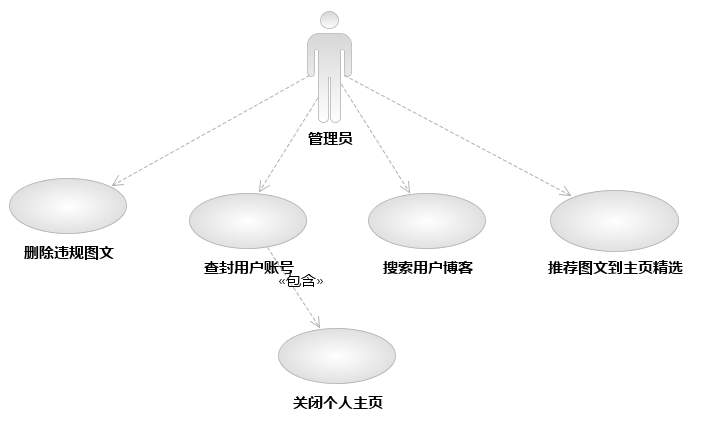
\includegraphics[width=4in]{用例图-管理员.jpeg}
\caption{用例图:管理员}
\label{fig:1}
\end{figure}

\begin{figure}[H]
\centering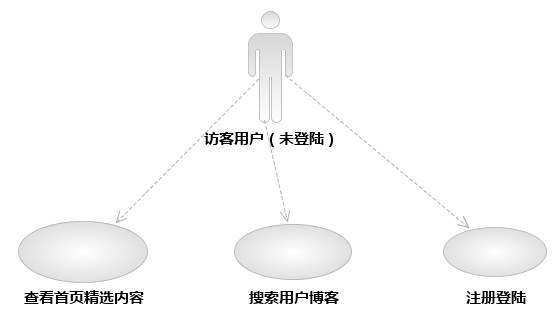
\includegraphics[width=4in]{用例图-访客.jpeg}
\caption{用例图:未登录用户}
\label{fig:2}
\end{figure}

\begin{figure}[H]
\centering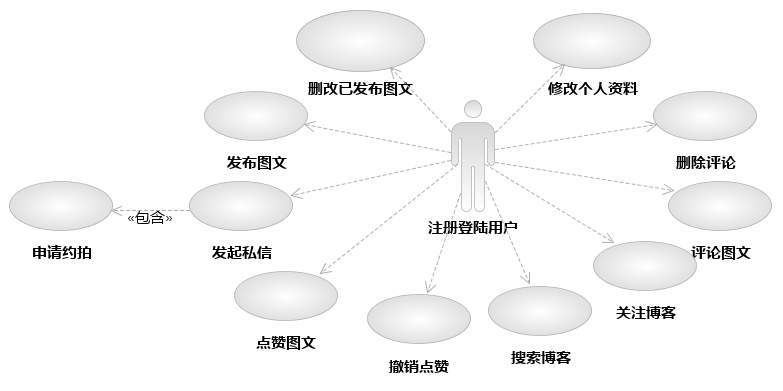
\includegraphics[width=4in]{用例图-用户.jpeg}
\caption{用例图:已登录用户}
\label{fig:3}
\end{figure}

\subsubsection{用户分类}
\begin{enumerate}[1)]
\item 摄影师\par
任意一个在网站申请为摄影师账号的用户,主要操作为搜索、发布图文
\item 模特\par
任意一个在网站申请为模特账号的用户,主要操作为搜索、发布图文
\item 管理员\par
这是一个专用账户,用于对网站内容进行监管,以及管理网站的后台运作,使网站正常运行
\end{enumerate}

\subsubsection{具体说明}
\begin{enumerate}[1)]
\item 摄影师\par
\begin{enumerate}[i]
\item 摄影师在注册时,必填信息包括所在城市、拍摄类型、成片风格、联系方式和价格范围。这些信息会显示在其个人主页的显眼位置
\item 已登陆的摄影师用户可以进入搜索页面,对其他摄影师或模特进行条件搜索
\item 摄影师用户可以关注其他摄影师或模特,也能被其他用户关注。在个人主页上,会显示其关注人数及粉丝数量
\item 对于已关注的其他用户所发布的图文,摄影师用户能够进行点赞和评论
\item 摄影师在主页能浏览以时间顺序排列的关注用户的图文信息,以及每日主页精选
\item 摄影师能编辑修改、删除其个人主页上已发布的图文

\end{enumerate}
\item 模特\par
\begin{enumerate}[i]
\item 模特在注册时,必填信息包括所在城市、拍摄类型、偏好风格、联系方式和收费标准。这些信息会显示在其个人主页的显眼位置
\item 已登陆的模特用户可以进入搜索页面,对其他摄影师或模特进行条件搜索
\item 模特用户可以关注其他摄影师或模特,也能被其他用户关注。在个人主页上,会显示其关注人数及粉丝数量
\item 对于已关注的其他用户所发布的图文,模特用户能够进行点赞和评论
\item 模特在主页能浏览以时间顺序排列的关注用户的图文信息,以及每日主页精选
\item 模特能编辑修改、删除其个人主页上已发布的图文

\end{enumerate}
\item 管理员\par
\begin{enumerate}[i]
\item 管理员能够查看所有已发布图文,但不能参与图文的评论和点赞等活动
\item 根据判断发布的图文信息是否符合互联信息管理规范及相关法律规定,管理员能够删除某条特定的图文发布
\item 	对于不符合互联网信息管理规范及相关法规的摄影师或模特的个人主页,管理员可以进行审查并查封。被查封的页面显示页面已被查封的文本信息,其中的图文信息都不能被访问及显示
\item 对于审核过程中遇到的优秀图文信息,管理员可以将其推送到首页推荐的轮播界面

\end{enumerate}
\end{enumerate}



\section{需求规定}
\subsection{对功能的规定}



\begin{enumerate}[1)]

\item 首页(未登录)
\begin{enumerate}[i]
\item 形式
	\begin{enumerate}[a)]
	\item 网页
\end{enumerate}
\item 内容
	\begin{enumerate}[a)]
\item  每日精选:为浏览者推荐的每日人气最高的图片,双击任一张图片打开该“图片模块”(见5))。
\item 登录,注册(见7)),登录/注册后进入已登录的首页(见2))。
\item 搜索按钮,点击打开新网页进入人物搜索页面(见3))。
\end{enumerate}
\end{enumerate}

\item 首页(已登录)
\begin{enumerate}[i]
\item 形式
	\begin{enumerate}[a)]
	\item 网页
\end{enumerate}
\item 内容
	\begin{enumerate}[a)]
\item  编辑模块(上传图片,编写文字,发布),发布的状态或图片以”个人模块“的形式出现在b所述图片/状态栏中。
\item 图片/状态栏:
\begin{itemize}
\item 个人模块\par
会员图标+会员id+图片模块+其他元素。若显示的是其他会员的图片或状态,则图片模块不可修改(见5))。若显示的是用户自身的图片或状态,则图片模块可修改(见6))。
\item 众多个人模块组成状态栏内容 \par
该内容展现“每日精选”,或展现“好友动态”。

\begin{figure}[H]
\centering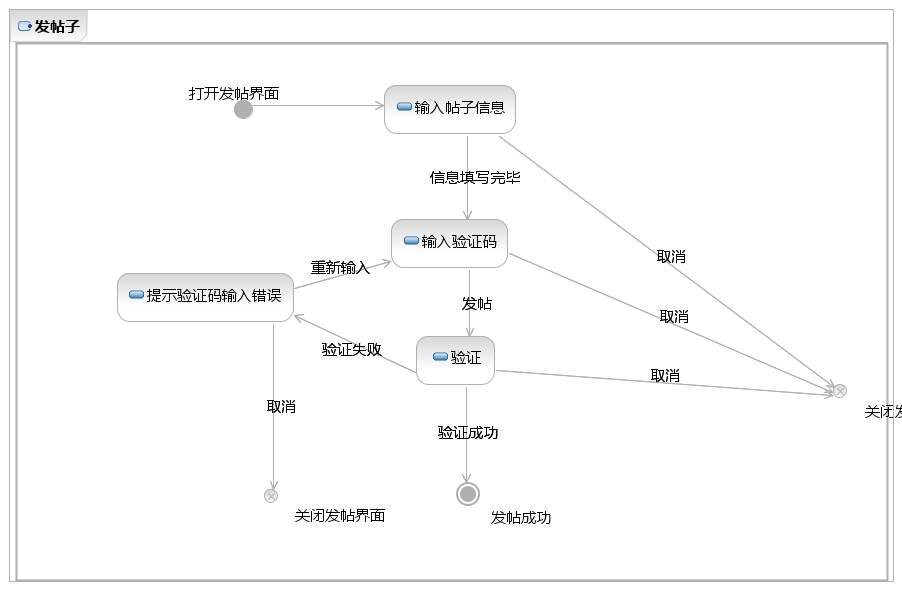
\includegraphics[width=4.5in]{状态图-发帖子.jpeg}
\caption{状态图:发帖子}
\label{fig:8}
\end{figure}

\end{itemize}

\end{enumerate}
\end{enumerate}

\begin{figure}[H]
\centering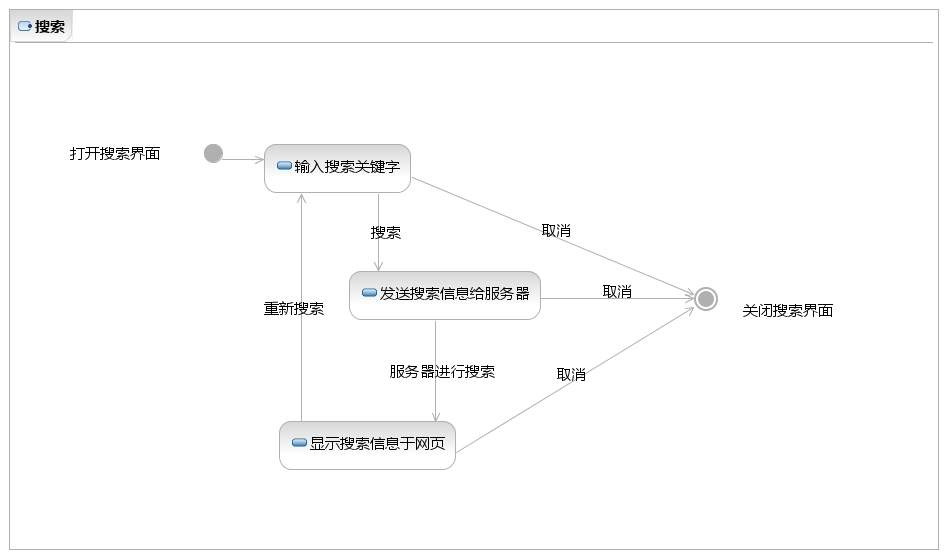
\includegraphics[width=4.5in]{状态图-搜索.jpeg}
\caption{状态图:搜索}
\label{fig:6}
\end{figure}

\item 人物搜索页面
\begin{enumerate}[i]
\item 形式
	\begin{enumerate}[a)]
\item 网页

	\end{enumerate}

\item 内容
 	\begin{enumerate}[a)]
	\item 搜索框和搜索按钮:在搜索框内输入会员id,点击搜索按钮搜索,搜索结果显示在“结果区域”中。
	\item 提供“综合” “人气” “风格” “类型”等下拉选项框(例如人气下拉选项有“大于500” 、“100-500” 、“<100”;类型下拉选项有“婚纱照”“艺术照”等)。浏览者(已登录或未登录)选择相应选项,系统给出符合要求的摄影师或模特的信息,结果显示在“结果区域”中。
	\item 结果区域:摄影师或模特的会员图标+id+简介+其他元素。点击某一元素可以打开新网页进入该会员个人主页

	\end{enumerate}
\end{enumerate}



\item 个人主页
\begin{enumerate}[i]
\item 形式
	\begin{enumerate}[a)]
	\item 网页

	\end{enumerate}

\item 内容
 	\begin{enumerate}[a)]
		\item 个人信息显示:显示个人简介,角色(摄影师,模特),联系方式,喜好,定价等。
\item 历史状态显示栏:由许多图片模块组成(不可修改)(见5))。
\item 私信:点击可发送短信给主页主人,条件是发起方是已登录的状态,主页主人自己不能发给自己。
\item 以上是其他用户访问可得到的信息,当已登录用户访问自己的主页时,拥有以下更多的元素:
\begin{itemize}
\item 个人信息编辑:用户点击某元素后以弹出框、侧拉框或新网页的形式编辑个人信息。
\item 历史状态显示栏显示的是可修改的图片模块。
\item c)中的私信变成“收件箱”,接收来自他人的私信,点击可查看。

\begin{figure}[H]
\centering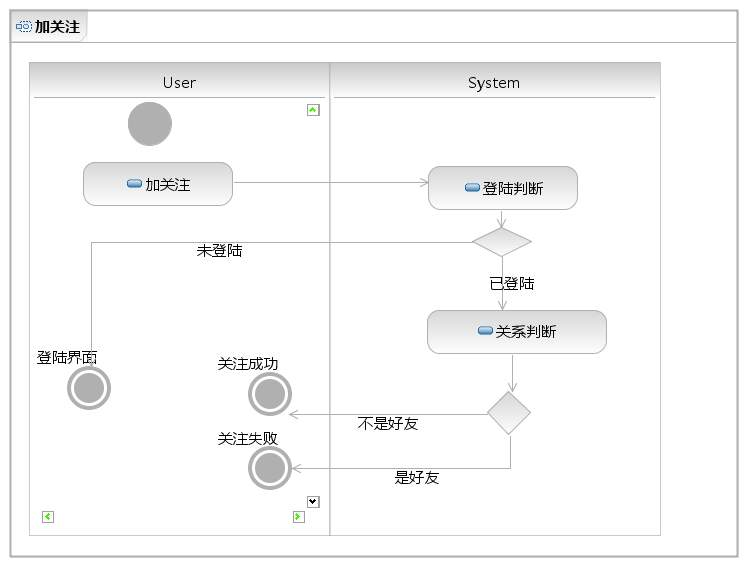
\includegraphics[width=4.5in]{活动图-加关注.jpeg}
\caption{活动图:添加关注}
\label{fig:13}
\end{figure}

\begin{figure}[H]
\centering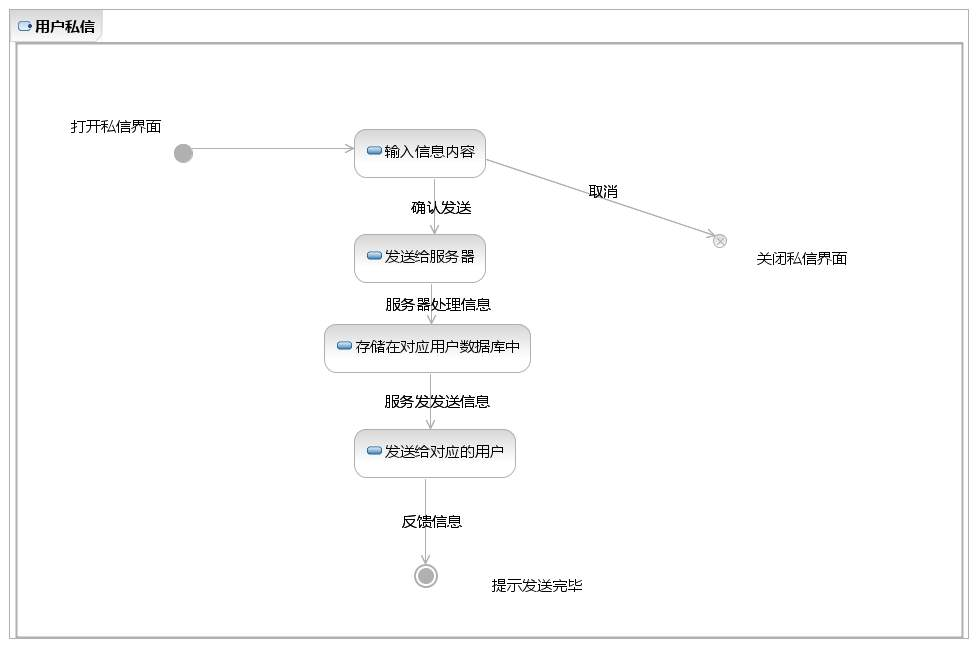
\includegraphics[width=4.5in]{状态图-私信.jpeg}
\caption{状态图:私信}
\label{fig:7}
\end{figure}

\end{itemize}


	\end{enumerate}
\end{enumerate}


\item 不可修改的图片模块
\begin{enumerate}[i]
\item 形式
	\begin{enumerate}[a)]
\item 作为html页面的一个元素或弹出窗口

	\end{enumerate}

\item 内容
 	\begin{enumerate}[a)]
\item 显示内容:图片缩略图/介绍/状态。
\item 评论:用户点击相关元素后可编辑对图片的评论并发布在该模块下,未登录的用户无法评论,但可以看到他人的评论。
\item 允许点赞,未登录的用户无法点赞,但可以看到点赞次数。

\begin{figure}[H]
\centering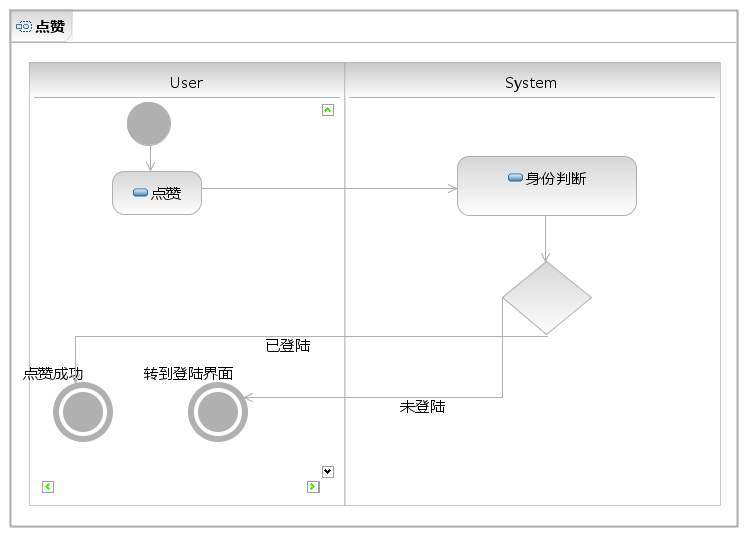
\includegraphics[width=4.5in]{活动图-点赞.jpeg}
\caption{活动图:点赞}
\label{fig:10}
\end{figure}

\begin{figure}[H]
\centering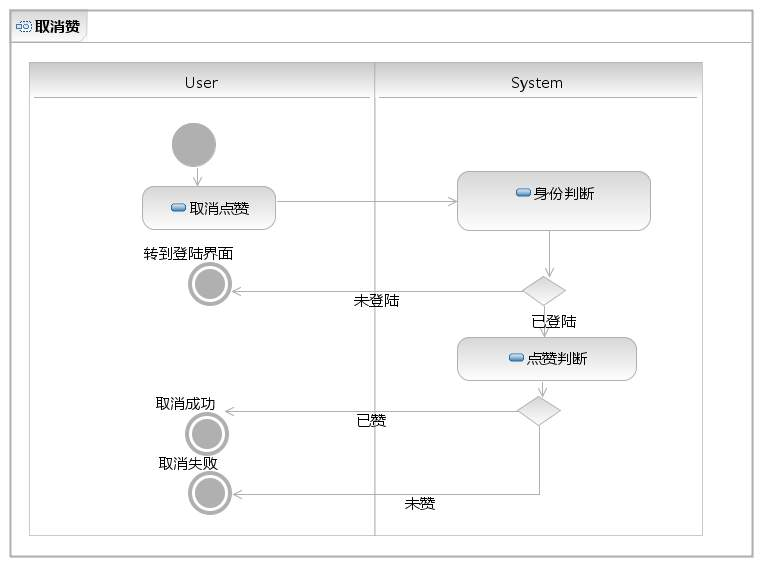
\includegraphics[width=4in]{活动图-取消赞.jpeg}
\caption{活动图:取消赞}
\label{fig:11}
\end{figure}

\begin{figure}[H]
\centering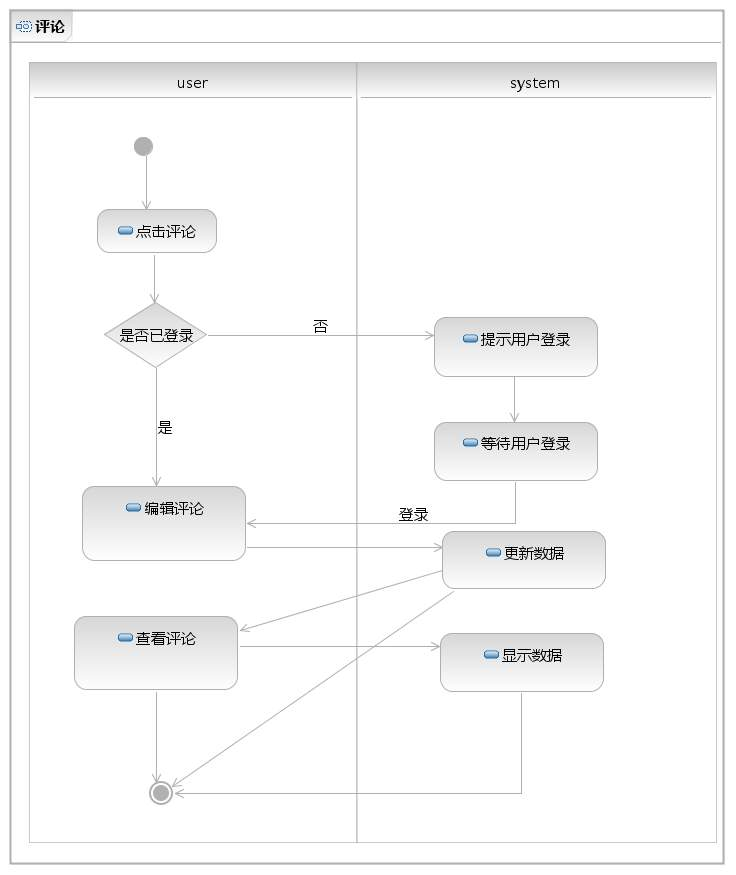
\includegraphics[width=4in]{活动图-评论.jpeg}
\caption{活动图:评论}
\label{fig:12}
\end{figure}

\item 查看大图:点击可查看放大的图片。
\item  标志:显示该图片是发布者作为“摄影师”还是作为“模特”参与制作的,系统会根据发布者角色(见7)c)自动标记,若发布者没指定或指定了两个角色,系统会在发布者发布时提醒其自行标记。



	\end{enumerate}
\end{enumerate}

\begin{figure}[H]
\centering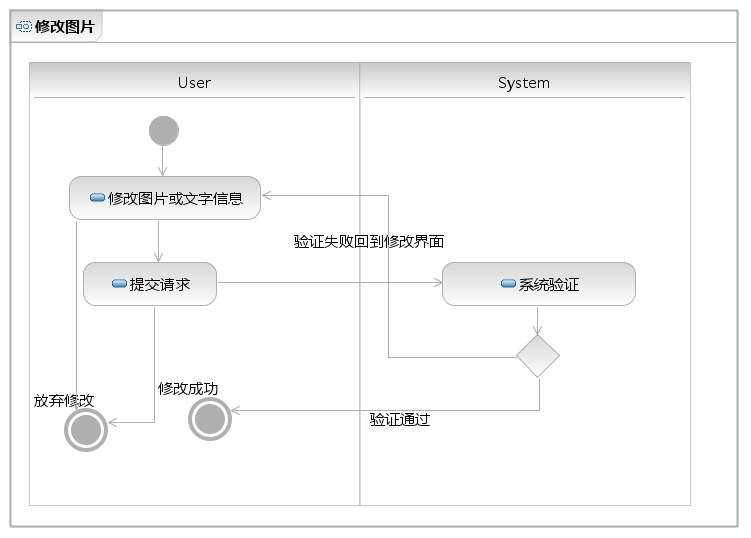
\includegraphics[width=4in]{活动图-修改图片.jpeg}
\caption{活动图:修改图片}
\label{fig:9}
\end{figure}

\item 可修改的图片模块 
\begin{enumerate}[i]
\item 形式
	\begin{enumerate}[a)]
\item 作为html页面的一个元素或弹出窗口

	\end{enumerate}

\item 内容\par
包含不可修改的图片模块的基本功能,以及如下功能:
 	\begin{enumerate}[a)]
\item 修改:修改内容,若修改后内容为空,则自动删除。
\item 删除:删除发布的状态或图片。




	\end{enumerate}
\end{enumerate}
\begin{figure}[H]
\centering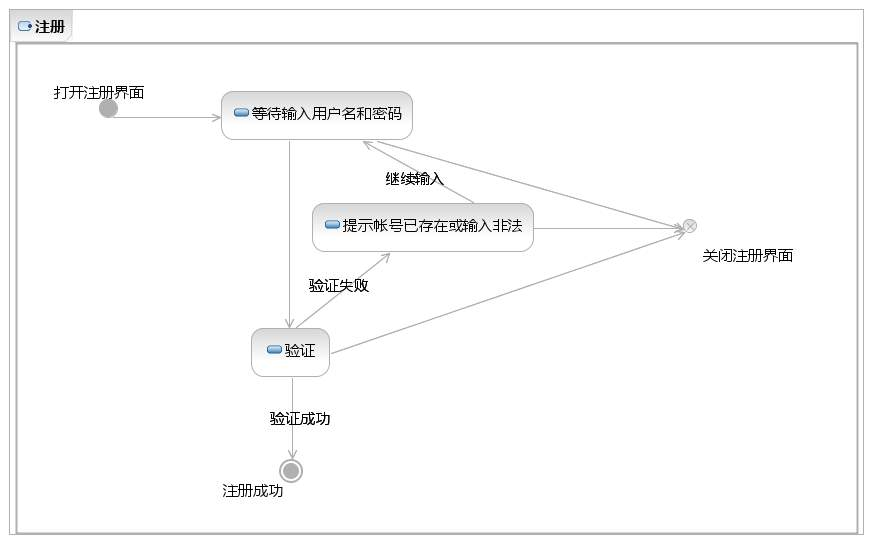
\includegraphics[width=4in]{状态图-注册.jpeg}
\caption{状态图:注册}
\label{fig:4}
\end{figure}

\begin{figure}[H]
\centering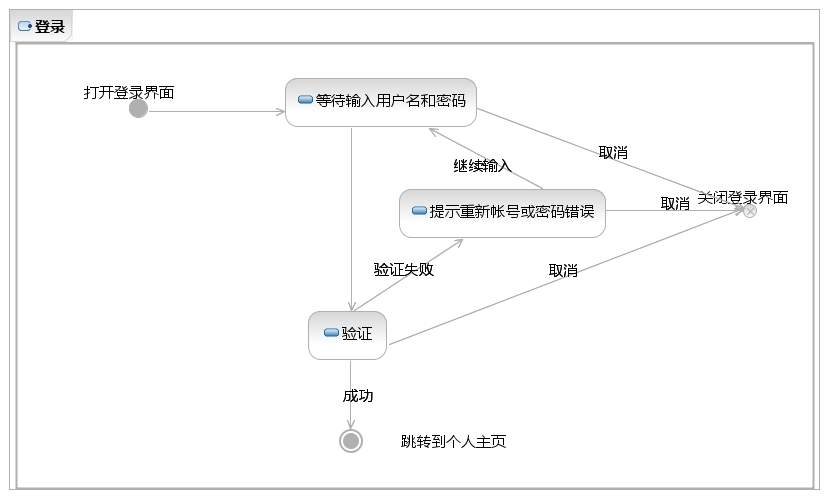
\includegraphics[width=4in]{状态图-登录.jpeg}
\caption{状态图:登录}
\label{fig:5}
\end{figure}
\item 登录和注册

\begin{figure}[H]
\centering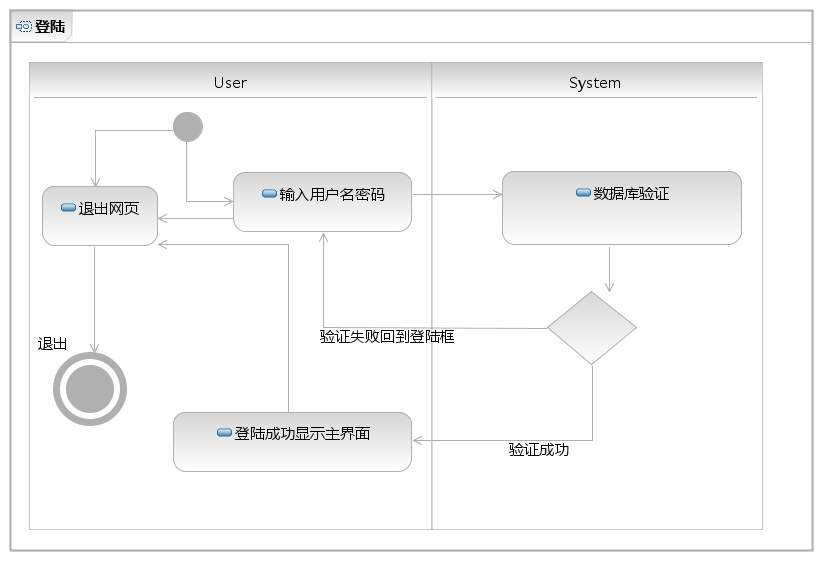
\includegraphics[width=4in]{活动图-登录.jpeg}
\caption{活动图:登录}
\label{fig:14}
\end{figure}

\begin{enumerate}[i]
\item 形式
	\begin{enumerate}[a)]
\item 作为每个网页的固有元素 + 弹出框

	\end{enumerate}

\item 内容\par
 	\begin{enumerate}[a)]
\item 如果用户已登录,显示用户id以及其他元素。
	\item 如果用户未登录,显示“登录”“注册”子样,点击登录或注册弹出信息填空框,用户填完信息并确认后即登录/注册成功。
	\item 注册信息时可以选定角色(摄影师、模特)或不选定。
  	\item 在用户所访问的页面中,用户登录与否都会以a、b的形式显示在当前页面中。
	\item 当未登录的用户执行需要会员权限的操作(如评论,私信)时,弹出登录信息填空框。




	\end{enumerate}
\end{enumerate}




\end{enumerate}


\subsection{对性能的规定}

\begin{figure}[H]
\centering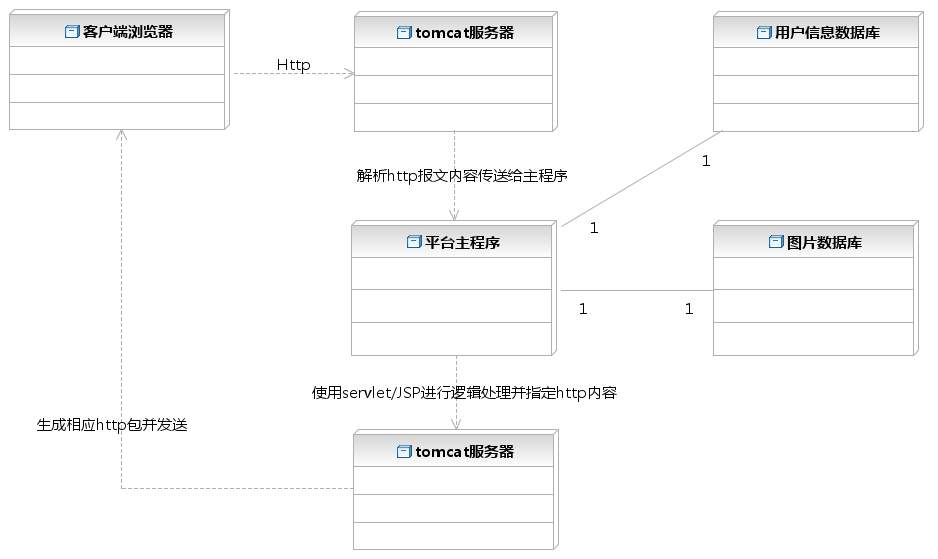
\includegraphics[width=4.5in]{部署图.jpeg}
\caption{部署图}
\label{fig:15}
\end{figure}

\subsubsection{时间特性要求}
\begin{enumerate}[1)]
\item 图片加载时间:网站以图片为主,图片加载速度直接影响用户体验。

\item 多个用户对并发操作时,后台处理一定要准确,同时要保证响应速度在可容忍范围内。


\end{enumerate}
\subsubsection{存储要求}
\begin{enumerate} [1)]
\item 图片占空间较大,后台数据存储空间要足够。

\item 后台数据需要备份。


\end{enumerate}
\subsubsection{灵活性}
\begin{enumerate} [1)]
\item 软件需求核心是用户发布的图片或状态。该软件将图片和相应的操作(添加,删除,评论)组成独立的模块,以适应用户需求的变更。
   

\item 软件前端采用html+css+javascript,可以用任意主流的浏览器(chrome,ie)打开;后端采用tomcat+jsp+sevlet+mysql,所用的技术比较通用,可以运行在主流的机器上。
    

\item  该软件目前作为“约拍”平台,在功能上可以进行延伸,变成图片分享交流交友的平台,届时只要增加或强化网站上互动的元素即可。
\end{enumerate}

\subsection{输入输出要求}
\begin{enumerate} [1)]
\item 注册输入 \par
\begin{itemize}
\item 昵称:6位以内字符
\item 账号:6-8位英文字符(大小写区分)
\item 密码:12位以内数字或英文
\item 邮箱(可选)
\item 头像:小于400k(图像压缩,可选)

\end{itemize}
注册成功进入主界面;失败则在原窗口弹出失败信息,要求用户修改后重新提交。

\item 登陆输入\par
输入账号/密码,登陆成功进入主界面;失败则在原窗口弹出失败信息,要求用户修改后重新提交。
\item  搜索输入 \par
模特、摄影师、图片的关键词 或者分类属性信息。成功输出搜索结果;失败显示无结果。
\item 私信输入 \par
聊天窗口输入字符串或者表情,聊天显示框输出双方实时聊天信息。
\item  状态发布输入 \par
输入图片及文字,勾选图片风格属性,发布成功进入主界面;失败则在原窗口弹出失败信息,要求用户修改后重新提交。

\end{enumerate}

\subsection{数据管理能力要求}
根据对用户上传图片的大小及数量,保证数据库系统稳定性。目前选定MySQL作为数据库。

\subsection{故障处理要求}
客户端硬件故障,用户根据具体pc的手册自行维护。\par
由于网络阻塞、请求冲突、服务器崩溃等原因,客户端web浏览器可能出现卡死,要求在前段实现时增强系统鲁棒性,实现对外部错误的反馈。 

%\subsection{其他专门要求}

\section{运行环境规定}
\subsection{设备}
最低配置:
\begin{itemize}
\item CPU PII-233MHz  
\item 128M内存  
\item 600MB硬盘空间   
\item 屏幕分辨率16bit 800×600  
\item 64K/bps以上的上网环境
\item 鼠标、键盘等外设正常
\end{itemize}
推荐配置:
\begin{itemize}
\item CPU PIII-500MHz 以上  
\item 256M 内存以上 
\item 800MB以上硬盘空间   
\item 屏幕分辨率16bit 1024*800
\item 2M宽带
\item 鼠标、键盘等外设正常
\end{itemize}

\subsection{支持软件}
\begin{itemize}
\item 操作系统:Windows/Linux/MacOS等均可
\item 编译(或汇编)程序:visual studio IDE内嵌汇编
\item 数据库:Mysql
\item 支持javascript的浏览器


\end{itemize}

\subsection{接口}
\begin{itemize}
\item 用户接口:\par
适用于 Internet Explorer 、Maxthon、 Mozilla Firefox、Opera 、Google Chrome 等主流 浏览器以及手机浏览器。
\item 数据通信协议:\par
\begin{enumerate}[1)]
\item UDP(User Datagram Protocol)用户数据报协议
\item TCP/IP(Transmission Control Protocol/Internet Protocol)传输控制协议/Internet 协议 
\item IPv4(Internet Protocol Version 4)Internet 协议-版本 4 
\item HTTP超文本传输协议 
\item FTP(File Transfer Protocol)文件传输协议 
\end{enumerate}

\end{itemize}

\section{UML模型附录}
\subsection{活动图}
\begin{figure}[H]
\centering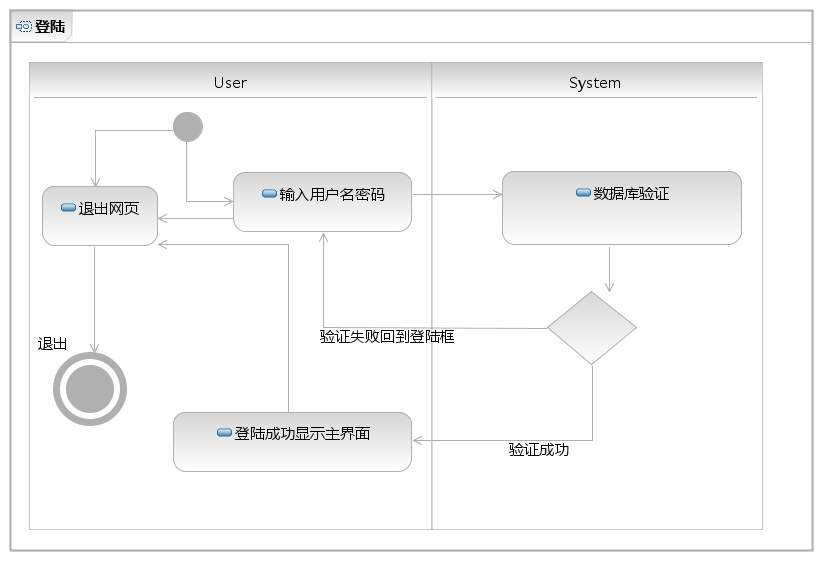
\includegraphics[width=4.5in]{活动图-登录.jpeg}
\caption{活动图:登录}
\end{figure}

\begin{figure}[H]
\centering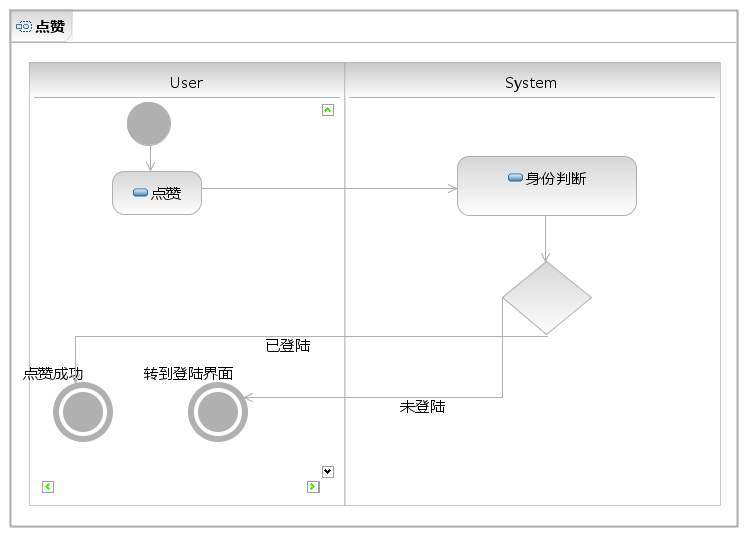
\includegraphics[width=4.5in]{活动图-点赞.jpeg}
\caption{活动图:点赞}
\end{figure}

\begin{figure}[H]
\centering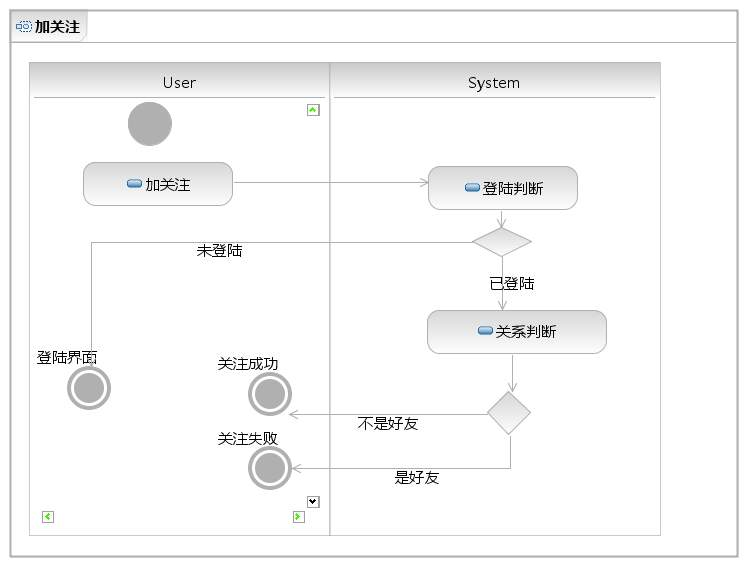
\includegraphics[width=4.5in]{活动图-加关注.jpeg}
\caption{活动图:加关注}
\end{figure}

\begin{figure}[H]
\centering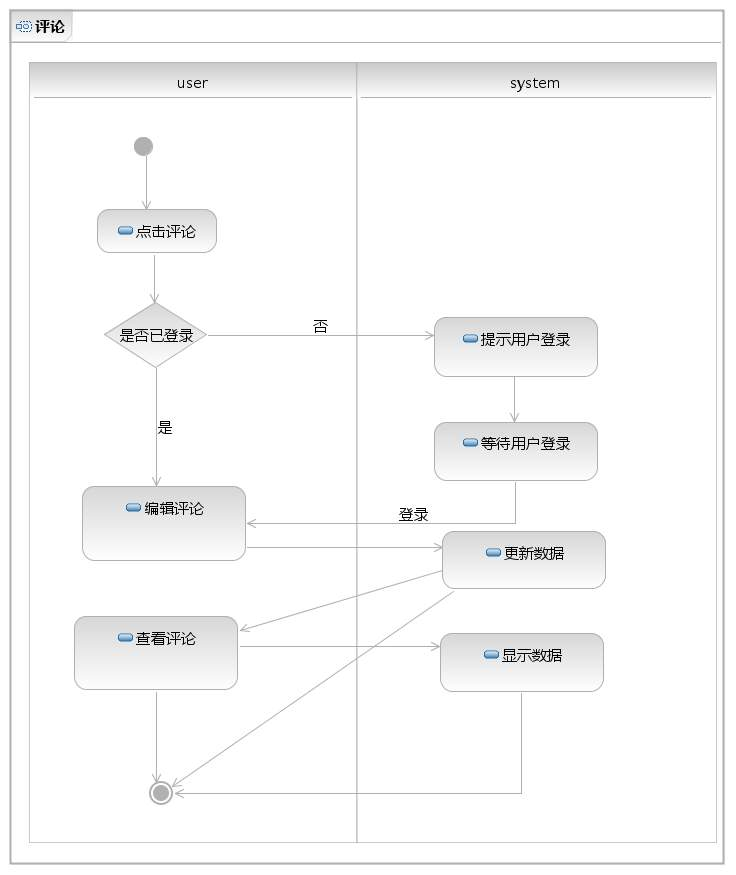
\includegraphics[width=4.5in]{活动图-评论.jpeg}
\caption{活动图:评论}
\end{figure}

\begin{figure}[H]
\centering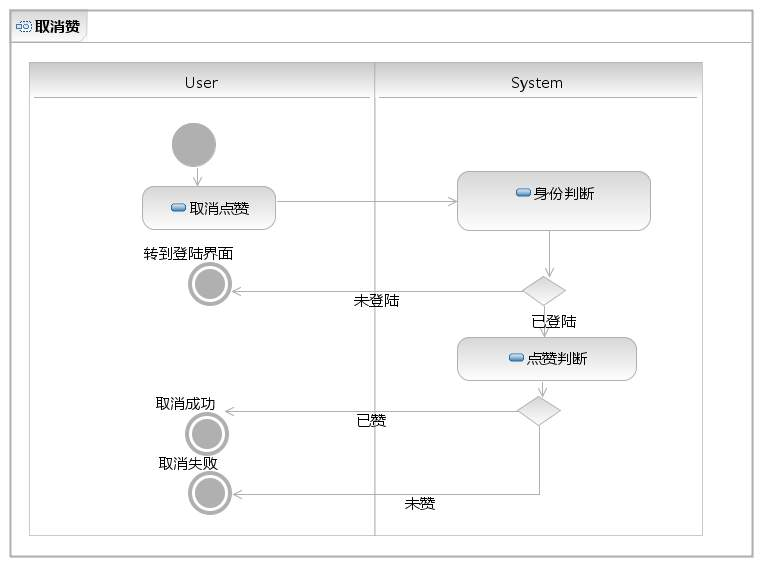
\includegraphics[width=4.5in]{活动图-取消赞.jpeg}
\caption{活动图:取消赞}
\end{figure}

\begin{figure}[H]
\centering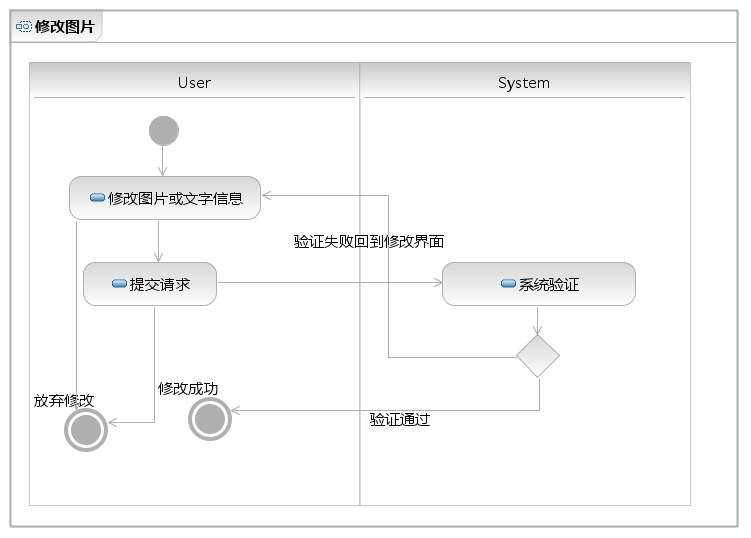
\includegraphics[width=4.5in]{活动图-修改图片.jpeg}
\caption{活动图:修改图片}
\end{figure}

\subsection{用例图}
\begin{figure}[H]
\centering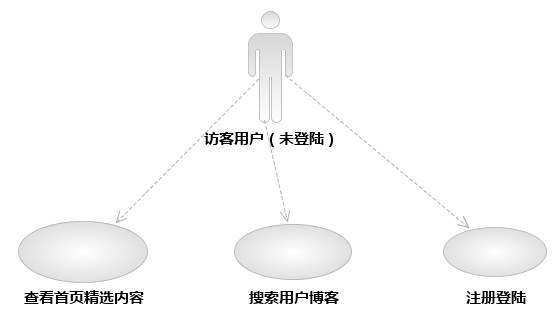
\includegraphics[width=4.5in]{用例图-访客.jpeg}
\caption{用例图:未登录用户}
\end{figure}

\begin{figure}[H]
\centering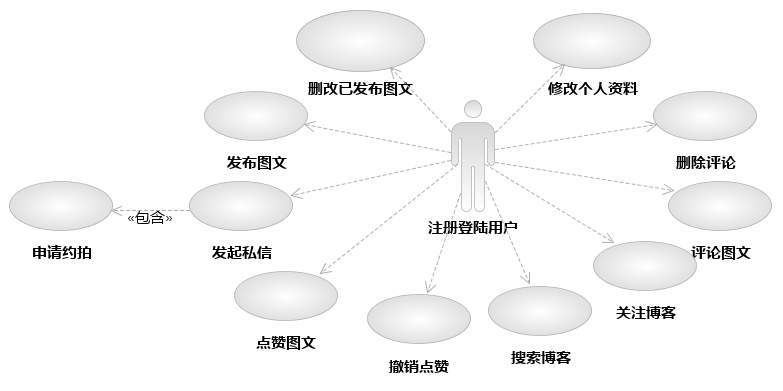
\includegraphics[width=4.5in]{用例图-用户.jpeg}
\caption{用例图:已登录用户}
\end{figure}

\begin{figure}[H]
\centering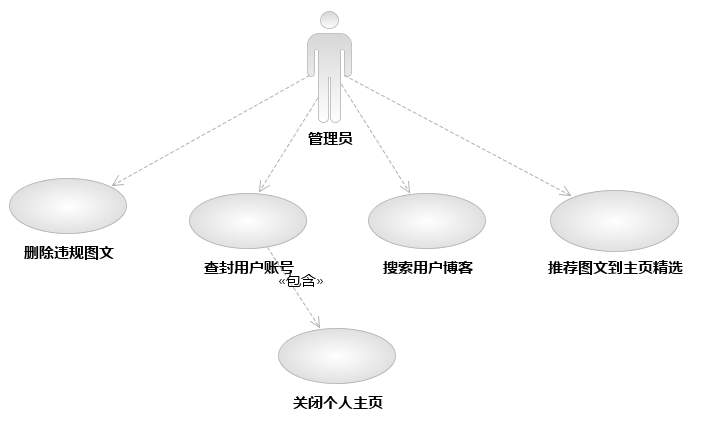
\includegraphics[width=4.5in]{用例图-管理员.jpeg}
\caption{用例图:管理员}
\end{figure}

\subsection{部署图}
\begin{figure}[H]
\centering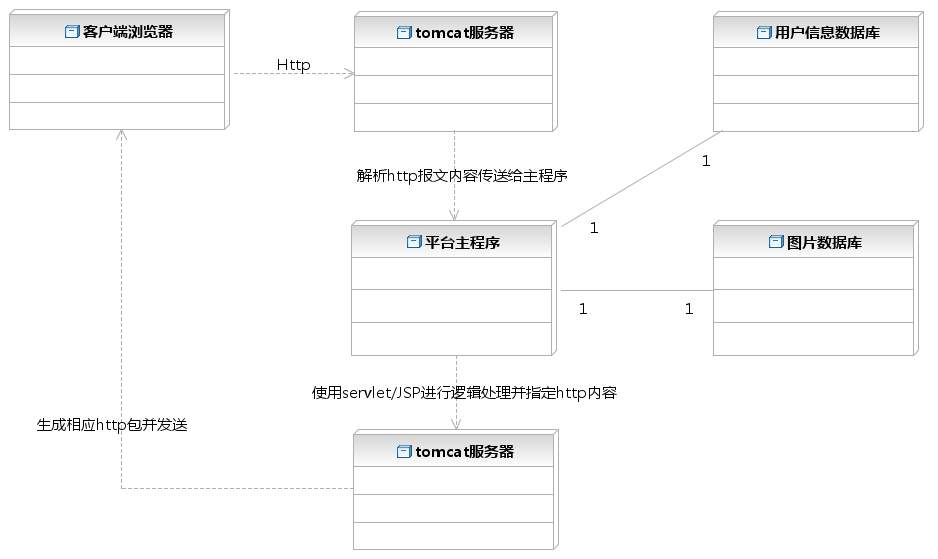
\includegraphics[width=4.5in]{部署图.jpeg}
\caption{部署图}
\end{figure}

\subsection{时序图}

\begin{figure}[H]
\centering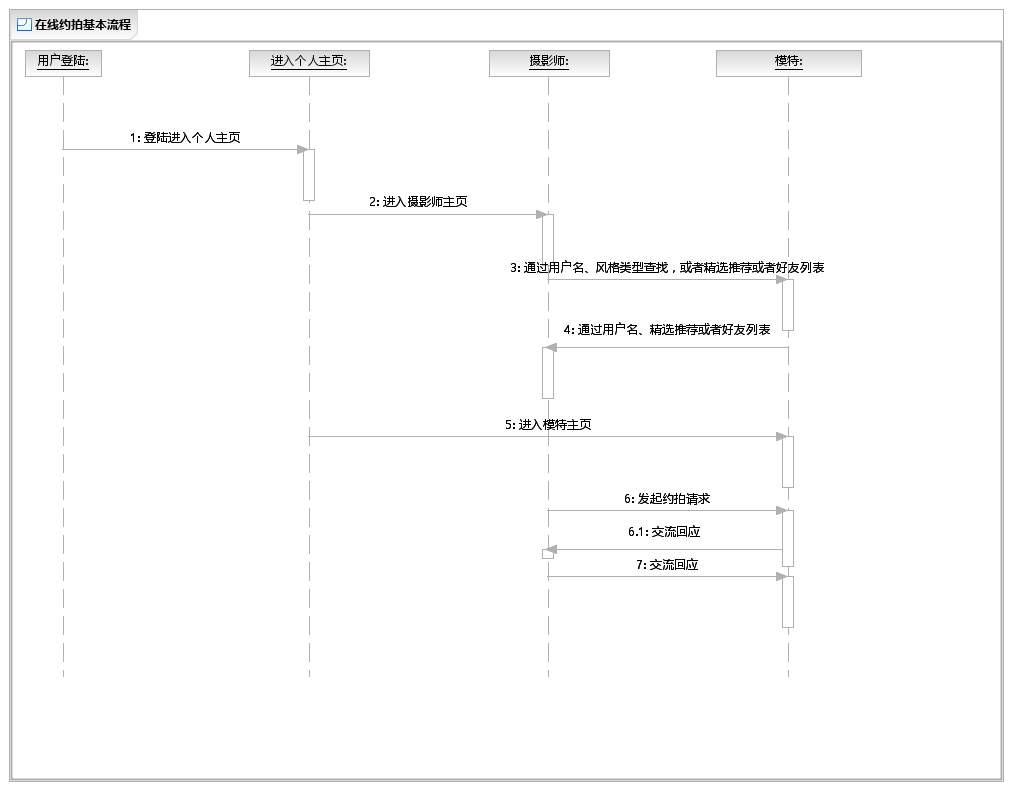
\includegraphics[width=4.5in]{时序图-约拍.jpeg}
\caption{时序图:约拍}
\end{figure}

\subsection{状态图}

\begin{figure}[H]
\centering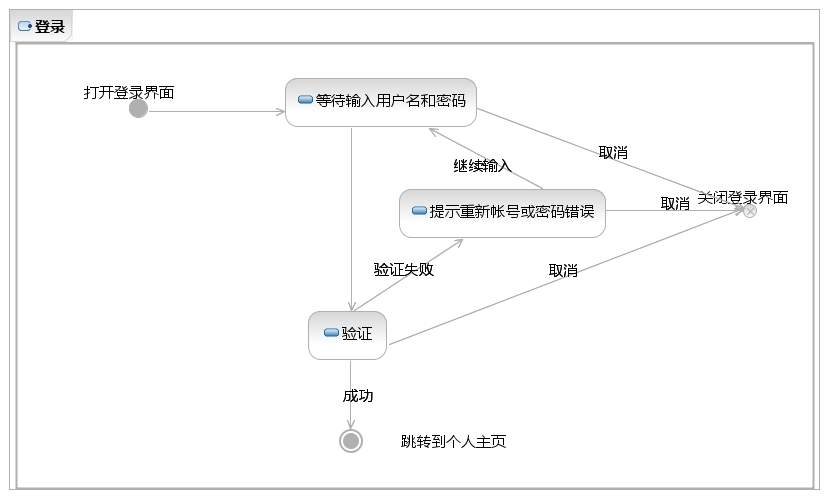
\includegraphics[width=4.5in]{状态图-登录.jpeg}
\caption{状态图:登录}
\end{figure}

\begin{figure}[H]
\centering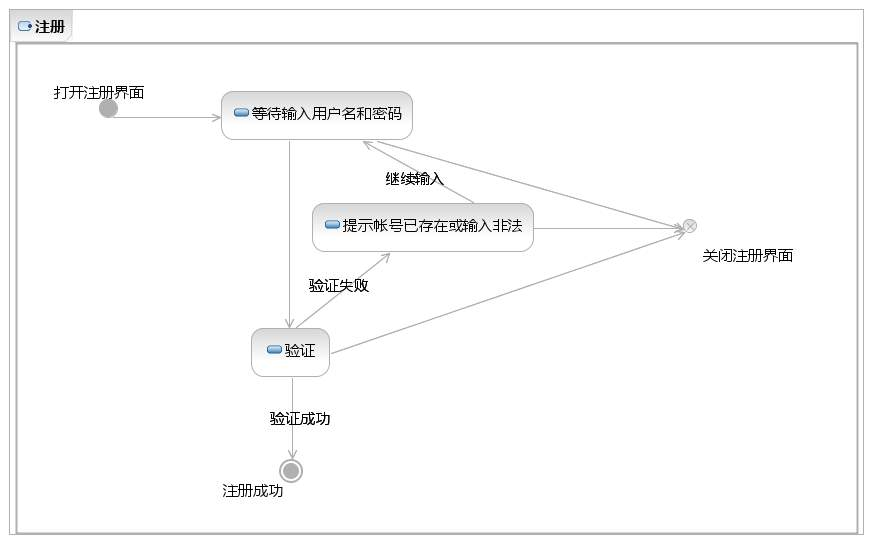
\includegraphics[width=4.5in]{状态图-注册.jpeg}
\caption{状态图:注册}
\end{figure}

\begin{figure}[H]
\centering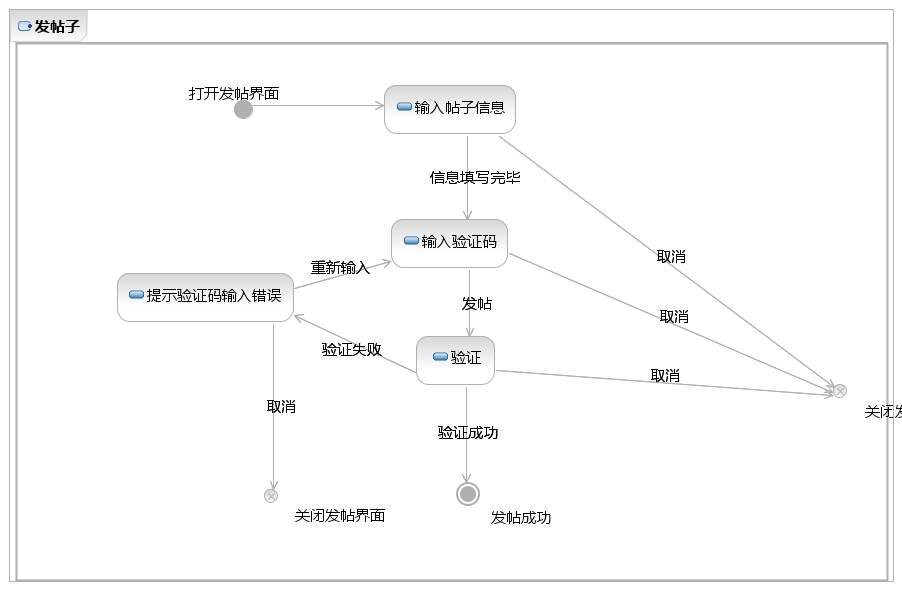
\includegraphics[width=4.5in]{状态图-发帖子.jpeg}
\caption{状态图:发帖子}
\end{figure}

\begin{figure}[H]
\centering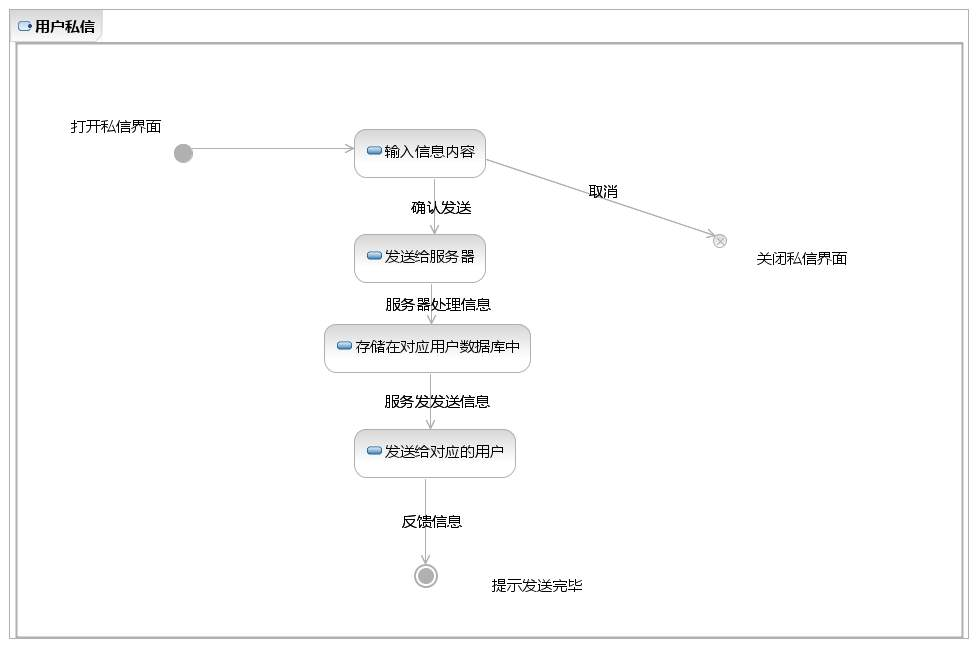
\includegraphics[width=4.5in]{状态图-私信.jpeg}
\caption{状态图:私信}
\end{figure}

\begin{figure}[H]
\centering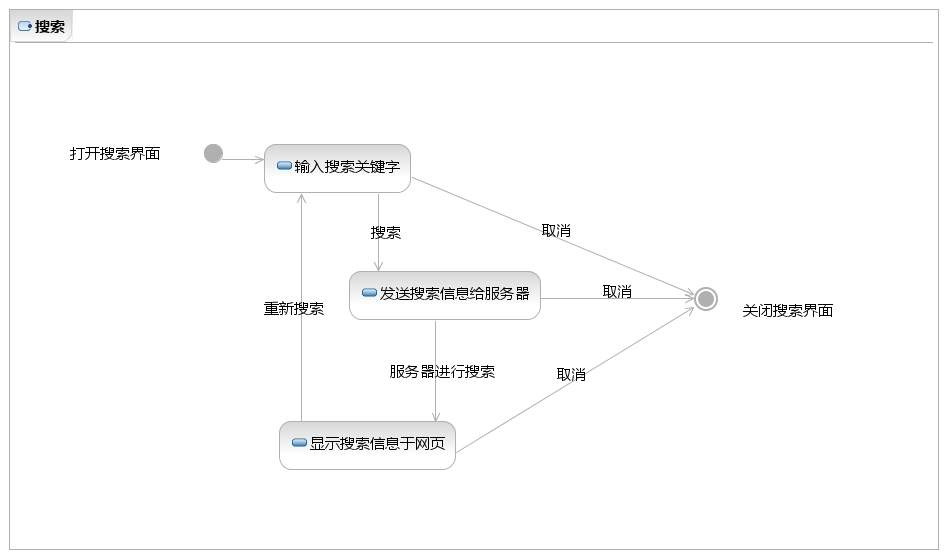
\includegraphics[width=4.5in]{状态图-搜索.jpeg}
\caption{状态图:搜索}
\end{figure}






\end{document}
